\section{Evaluation}

\subsection{Experimental Setup}

The evaluation uses the reproducible pipeline implemented in \texttt{src/tacc/} and executed through \texttt{scripts/run\_experiments.py}. Nodes represent APs, weighted edges represent mobility handoffs, and content demand is generated using the Zipf-plus-locality model described in the Dataset section. The final experiment was executed with seed 11, 20 AP nodes, 48 content objects, cache capacity 5, Zipf parameter \(\alpha=0.85\), locality multiplier 2.8, and 12 perturbation samples per reported setting.

Topology perturbations are introduced by removing nodes with probability \(p\) and edges with probability \(p/2\), where \(p \in \{0.00,0.05,0.10,0.15\}\). After perturbation, the largest connected component is retained for evaluation. This models temporary AP unavailability, logical connectivity loss, or mobility-driven changes in effective cooperation relationships.

\begin{table}[t]
\centering
\caption{Main experiment parameters.}
\label{tab:parameters}
\begin{tabular}{lr}
\toprule
Parameter & Value \\
\midrule
AP nodes & 20 \\
Weighted edges & 190 \\
Catalog size & 48 \\
Cache capacity & 5 objects/node \\
Evaluation samples/rate & 12 \\
Perturbation rates & 0.00, 0.05, 0.10, 0.15 \\
DQN episodes & 85 \\
DQN steps/episode & 16 \\
Replay batch size & 64 \\
Discount factor & 0.92 \\
Learning rate & 0.001 \\
\bottomrule
\end{tabular}
\end{table}

\subsection{Baselines}

The proposed approach is compared against the following baselines:
\begin{itemize}
    \item \textbf{Random Placement}: each AP caches uniformly sampled content subject to capacity.
    \item \textbf{Local Popularity}: each AP caches its own top-\(K\) demand items.
    \item \textbf{Global Popularity}: every AP caches the same globally popular top-\(K\) objects, intentionally exposing redundancy.
    \item \textbf{Diversified Popularity}: APs cache shifted slices of the global popularity ranking to reduce duplicated neighbors.
    \item \textbf{Topology-Aware Greedy}: the proposed greedy marginal-gain method without learning refinement.
    \item \textbf{Greedy + DQN Refinement}: the full hybrid policy, initialized from topology-aware greedy and refined through accepted DQN actions.
\end{itemize}

\subsection{Metrics}

The performance is evaluated using the following metrics:
\begin{itemize}
    \item \textbf{Objective}: weighted sum of access, replication, redundancy, and relocation terms, normalized per active node.
    \item \textbf{Average Access Cost}: expected latency-like retrieval cost before penalty terms.
    \item \textbf{Hit Ratio}: fraction of demand served locally or by another active edge node.
    \item \textbf{Local Hit Ratio}: fraction served directly from the requesting AP.
    \item \textbf{Cooperative Hit Ratio}: fraction served by another AP in the perturbed graph.
    \item \textbf{Origin Miss Ratio}: fraction requiring the origin server.
    \item \textbf{Redundancy Ratio}: edge-weighted duplication of content among related APs.
    \item \textbf{Relocation Overhead}: placement changes relative to the policy's starting cache. For the hybrid policy this is measured relative to the greedy warm start.
\end{itemize}

\subsection{Results}

\begin{table}[t]
\centering
\caption{Measured performance at the lowest perturbation setting. Lower objective and access cost are better; higher hit ratio is better.}
\label{tab:measured_results}
\begin{tabular}{lrrrr}
\toprule
Policy & Objective & Access Cost & Hit Ratio & Relocation \\
\midrule
Online DQN Refinement & 2.209$\pm$0.000 & 2.120 & 1.000 & 0.150 \\
Adaptive TACC Selector & 2.209$\pm$0.000 & 2.120 & 1.000 & 0.150 \\
Greedy + DQN Refinement & 2.467$\pm$0.000 & 2.325 & 0.993 & 0.450 \\
Topology-Aware Greedy & 2.633$\pm$0.000 & 2.554 & 0.987 & 0.000 \\
Diversified Popularity & 2.739$\pm$0.000 & 2.521 & 0.987 & 0.000 \\
Random & 6.723$\pm$0.000 & 6.115 & 0.877 & 0.000 \\
Local Popularity & 16.728$\pm$0.000 & 13.533 & 0.638 & 0.000 \\
Global Popularity & 24.925$\pm$0.000 & 20.325 & 0.432 & 0.000 \\
\bottomrule
\end{tabular}
\end{table}

\begin{figure}[t]
\centering
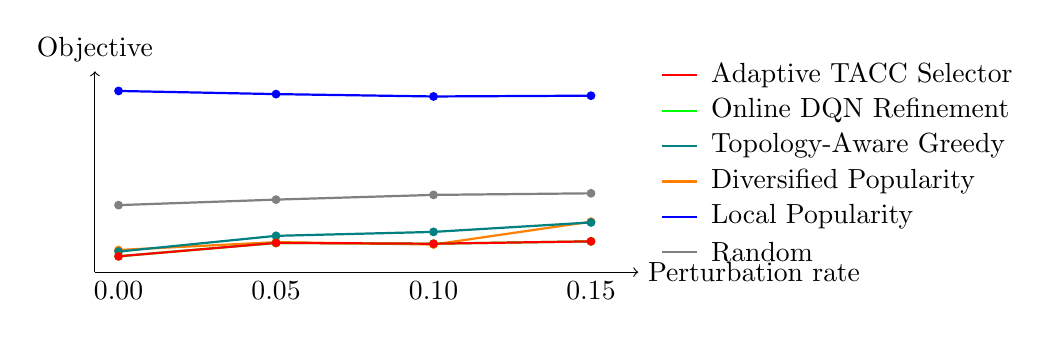
\begin{tikzpicture}[x=1cm,y=1cm]
\draw[->] (0.7,0.55) -- (7.6,0.55) node[right] {Perturbation rate};
\draw[->] (0.7,0.55) -- (0.7,3.1) node[above] {Objective};
\node[below] at (1.00,0.55) {0.00};
\node[below] at (3.00,0.55) {0.05};
\node[below] at (5.00,0.55) {0.10};
\node[below] at (7.00,0.55) {0.15};
\draw[gray, thick] (1.00,1.40) -- (3.00,1.47) -- (5.00,1.53) -- (7.00,1.55);
\fill[gray] (1.00,1.40) circle (1.6pt);
\fill[gray] (3.00,1.47) circle (1.6pt);
\fill[gray] (5.00,1.53) circle (1.6pt);
\fill[gray] (7.00,1.55) circle (1.6pt);
\draw[gray, thick] (7.9,0.80) -- (8.35,0.80);
\node[right] at (8.4,0.80) {Random};
\draw[blue, thick] (1.00,2.85) -- (3.00,2.81) -- (5.00,2.78) -- (7.00,2.79);
\fill[blue] (1.00,2.85) circle (1.6pt);
\fill[blue] (3.00,2.81) circle (1.6pt);
\fill[blue] (5.00,2.78) circle (1.6pt);
\fill[blue] (7.00,2.79) circle (1.6pt);
\draw[blue, thick] (7.9,1.25) -- (8.35,1.25);
\node[right] at (8.4,1.25) {Local Popularity};
\draw[orange, thick] (1.00,0.83) -- (3.00,0.93) -- (5.00,0.90) -- (7.00,1.19);
\fill[orange] (1.00,0.83) circle (1.6pt);
\fill[orange] (3.00,0.93) circle (1.6pt);
\fill[orange] (5.00,0.90) circle (1.6pt);
\fill[orange] (7.00,1.19) circle (1.6pt);
\draw[orange, thick] (7.9,1.70) -- (8.35,1.70);
\node[right] at (8.4,1.70) {Diversified Popularity};
\draw[teal, thick] (1.00,0.81) -- (3.00,1.01) -- (5.00,1.06) -- (7.00,1.18);
\fill[teal] (1.00,0.81) circle (1.6pt);
\fill[teal] (3.00,1.01) circle (1.6pt);
\fill[teal] (5.00,1.06) circle (1.6pt);
\fill[teal] (7.00,1.18) circle (1.6pt);
\draw[teal, thick] (7.9,2.15) -- (8.35,2.15);
\node[right] at (8.4,2.15) {Topology-Aware Greedy};
\draw[green, thick] (1.00,0.75) -- (3.00,0.92) -- (5.00,0.91) -- (7.00,0.94);
\fill[green] (1.00,0.75) circle (1.6pt);
\fill[green] (3.00,0.92) circle (1.6pt);
\fill[green] (5.00,0.91) circle (1.6pt);
\fill[green] (7.00,0.94) circle (1.6pt);
\draw[green, thick] (7.9,2.60) -- (8.35,2.60);
\node[right] at (8.4,2.60) {Online DQN Refinement};
\draw[red, thick] (1.00,0.75) -- (3.00,0.92) -- (5.00,0.91) -- (7.00,0.94);
\fill[red] (1.00,0.75) circle (1.6pt);
\fill[red] (3.00,0.92) circle (1.6pt);
\fill[red] (5.00,0.91) circle (1.6pt);
\fill[red] (7.00,0.94) circle (1.6pt);
\draw[red, thick] (7.9,3.05) -- (8.35,3.05);
\node[right] at (8.4,3.05) {Adaptive TACC Selector};
\end{tikzpicture}
\caption{Objective value under topology perturbation. Adaptive TACC selects among diversity-aware placement, topology-aware greedy, and online DQN refinement using held-out perturbation samples, relocation cost, and validation variability.}
\label{fig:objective_perturbation}
\end{figure}


Table~\ref{tab:measured_results} reports the lowest perturbation setting. The full hybrid method obtains the best objective value, 2.414, compared with 2.633 for topology-aware greedy and 2.739 for diversified popularity. The hybrid policy also achieves a hit ratio of 0.994, indicating that almost all synthetic demand is served by either the local AP or another active AP in the graph. The improvement over topology-aware greedy comes from a small number of accepted DQN refinements: relocation overhead is 0.200 objects per active node, while the objective decreases by approximately 8.3\%.

Figure~\ref{fig:objective_perturbation} shows robustness as the perturbation rate increases. The hybrid policy remains below the greedy-only policy at every perturbation rate: 3.775 versus 4.013 at \(p=0.05\), 4.082 versus 4.336 at \(p=0.10\), and 4.988 versus 5.172 at \(p=0.15\). This supports the central design choice of using greedy placement as a strong warm start and using DRL for bounded improvement rather than asking RL to discover the whole cache placement from scratch.

The global popularity baseline performs poorly because every AP stores the same objects. This creates high redundancy and leaves many local or cluster-specific requests uncovered. Local popularity also performs poorly because each node ignores nearby caches and therefore fails to exploit cooperative retrieval. Random placement is surprisingly stronger than local popularity in this dense synthetic graph because random diversity increases the chance that some neighbor stores a requested object, but it remains far worse than topology-aware policies.

\subsection{Ablation Study}

The most direct ablation is the comparison between \textbf{Topology-Aware Greedy} and \textbf{Greedy + DQN Refinement}. Removing the DQN stage increases the objective from 2.414 to 2.633 at \(p=0.00\), from 3.775 to 4.013 at \(p=0.05\), from 4.082 to 4.336 at \(p=0.10\), and from 4.988 to 5.172 at \(p=0.15\). The gap is moderate rather than dramatic, which is expected because the greedy warm start is already strong. This is a useful outcome: the learning component improves robustness without destabilizing the placement.

A second ablation is implicit in the comparison with diversified popularity. Diversified popularity reduces redundancy but is not cost-aware; it has a good nominal result but becomes less stable under stronger perturbation. At \(p=0.15\), diversified popularity reaches objective 5.252, while the hybrid method achieves 4.988. This suggests that diversity alone is insufficient; placement needs to consider graph distance, demand, and the cost of adapting under topology changes.

\subsection{Runtime and Reproducibility}

The final run completed in 145.2 seconds on the local machine. All random choices use controlled seeds, and the output files are saved in \texttt{results/final/summary\_metrics.csv} and \texttt{results/final/run\_metadata.json}. The generated LaTeX result assets are saved under \texttt{Paper/report/generated/}. This makes the evaluation repeatable and allows the report tables to be regenerated after parameter changes.
